\documentclass{beamer}

\usecolortheme[light]{solarized}

\beamertemplatenavigationsymbolsempty

\usepackage{hyperref}
\usepackage{minted}

\usepackage{graphicx}
\usepackage{tikz}

\usetikzlibrary{calc, patterns}

\begin{document}

    \begin{frame}
        \begin{center}
            \Huge

            Why you are here.

            \vspace{1cm}
            \Large

            \begin{columns}
                \begin{column}{.3\textwidth}
                    \href{https://twitter.com/drvinceknight}
                    {@drvinceknight}
                \end{column}


                \begin{column}{.3\textwidth}
                    \href{https://github.com/opcambell}
                    {@opcambell}
                \end{column}

                \begin{column}{.3\textwidth}
                    \href{https://github.com/alexwlchan}
                    {@alexwlchan}
                \end{column}

            \end{columns}

        \end{center}
    \end{frame}

    \begin{frame}
            \begin{columns}
                \begin{column}{.5\textwidth}
                    \begin{center}
                        
\includegraphics[width=3cm]{./static/CUident_CMYK.eps}
                    \end{center}
                \end{column}
                \begin{column}{.5\textwidth}
                    \begin{center}
                        
\includegraphics[width=3cm]{./static/pycon_uk.png}
                    \end{center}
                \end{column}
            \end{columns}

            \begin{columns}
                \begin{column}{.5\textwidth}
                    \begin{center}
                        
\includegraphics[width=3cm]{./static/PyDiff_logo.png}
                    \end{center}
                \end{column}
                \begin{column}{.5\textwidth}
                    \begin{center}
                        
\includegraphics[width=3cm]{./static/axelrod_logo.png}
                    \end{center}
                \end{column}
            \end{columns}
    \end{frame}


    \begin{frame}
        \begin{center}
            David MacIver - \url{Hypothesis.works} -
            \href{https://twitter.com/DRMacIver}{@DRMacIver} 


            \vspace{1cm}
            \url{http://bit.ly/hard-problems}
        \end{center}
    \end{frame}

    \begin{frame}
        \[
            \text{maximise: }16 x + 10 y
        \]
        such that:
        \begin{align*}
            2 x + y   &\leq 4 \\
            2 x + 2 y &\leq 6 \\
            x         &\geq 0 \\
            y         &\geq 0 \\
        \end{align*}
    \end{frame}

    \begin{frame}
        \begin{center}
            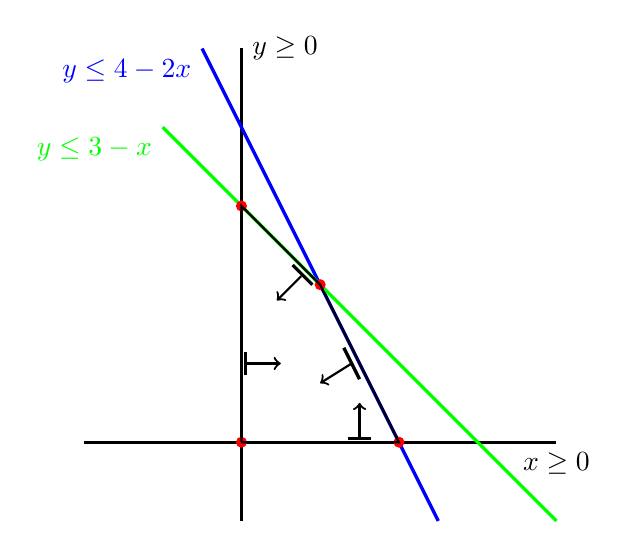
\begin{tikzpicture}
                % x >= 0
                \onslide<1-2>{
                \draw [very thick] (-2, 0) -- (4, 0)
                    node [pos=1, below] {\(x\geq 0\)};
                \draw [black, ->, thick] (1.5, 0.05) -- (1.5, .5);
                \draw [black, very thick] (1.35, 0.05) -- (1.65, 0.05);

                % y >= 0
                \draw [very thick] (0, -1) -- (0, 5)
                    node [pos=1, right] {\(y \geq 0\)};
                \draw [black, ->, thick] (0.05, 1) -- (.5, 1);
                \draw [black, very thick] (0.05, .85) -- (0.05, 1.15);

                % Draw y = 4 - 2 x
                \draw [very thick, blue] (-0.5, 5) -- (2.5, -1)
                    node [pos=0, below left] {\(y \leq 4 - 2 x\)};
                \draw [black, thick, ->] (1.4, 1) -- (1, 0.75);
                \draw [black, very thick] (1.3, 1.2) -- (1.5, 0.8);

                % Draw y = 3 - x
                \draw [very thick, green] (-1, 4) -- (4, -1)
                    node [pos=0, below left] {\(y \leq 3 - x\)};
                \draw [black, ->, thick] (0.76, 2.11) -- (.45, 1.8);
                \draw [black, very thick] (.9, 2) -- (.65, 2.25);
                }   

                % Vertices
                \onslide<2-3>{
                \fill [red] (0, 0)  circle[radius=2pt];
                \fill [red] (2, 0)  circle[radius=2pt];
                \fill [red] (0, 3)  circle[radius=2pt];
                \fill [red] (1, 2)  circle[radius=2pt];
                }   

                % polygon
                \onslide<3>{
                \draw [thick] (0, 0) -- (2, 0) -- (1, 2) -- (0, 3) -- (0, 0);
                }

            \end{tikzpicture}
        \end{center}
    \end{frame}

    \begin{frame}[fragile]{}
        \begin{minted}{python}
>>> import numpy as np
>>> import scipy as sp
>>> assert sp.__version__ == '0.19.0'
>>> from scipy import spatial
>>> halfspaces = np.array([[2, 1, -4], 
...                        [2, 2, -6],
...                        [-1, 0, 0],
...                        [0, -1, 0]])
>>> feasible_point = np.array([1/2, 1/2])
>>> hs = spatial.HalfspaceIntersection(
...     halfspaces=halfspaces, 
...     interior_point=feasible_point)
>>> hs.intersections
array([[ 0.,  0.],
       [ 2.,  0.],
       [ 0.,  3.],
       [ 1.,  2.]])

        \end{minted}
\end{frame}

    \begin{frame}
        \Large
        \[
            X = 
            \begin{pmatrix}
                1 & 0 & 0 & 0 & 0 & 0 & 0 & 0\\
                0 & 0 & 1 & 0 & 0 & 0 & 0 & 0\\
                0 & 1 & 0 & 0 & 0 & 0 & 0 & 0\\
                0 & 0 & 0 & 0 & 1 & 0 & 0 & 0\\
                0 & 0 & 0 & 0 & 0 & 1 & 0 & 0\\
                0 & 0 & 0 & 1 & 0 & 0 & 0 & 0\\
            \end{pmatrix}
        \]

        \[
           \sum_{\text{columns}}X_{ij} = 1 \qquad
           \sum_{\text{rows}}X_{ij} \leq 1
        \]
    \end{frame}

    \begin{frame}
        \Large
        \begin{center}
            \href{http://conference-scheduler.readthedocs.io/}
                 {conference-scheduler.readthedocs.io/}
        \end{center}
    \end{frame}

    \begin{frame}[fragile]{}
        \begin{minted}{python}
>>> from conference_scheduler.resources import Slot, Event
        \end{minted}
\end{frame}

    \begin{frame}
        \Huge
        \begin{center}
            Physics
        \end{center}
    \end{frame}

    \begin{frame}
        \Large  
        \[
            C_s = 
            \begin{pmatrix}
                1 & 1 & 1 & 1 & 1 & 1 & 1 & 1 \\
                1 & 1 & 0 & 0 & 1 & 1 & 1 & 1\\
                1 & 1 & 0 & 0 & 1 & 1 & 1 & 1\\
                1 & 1 & 1 & 1 & 1 & 0 & 1 & 1\\
                1 & 1 & 1 & 1 & 1 & 1 & 1 & 1\\
                1 & 1 & 1 & 1 & 1 & 1 & 1 & 1\\
            \end{pmatrix}
        \]

        \[
        X_{ij} \leq {C_{s}}_{ij}
        \]
    \end{frame}

    \begin{frame}
        \Huge
        \begin{center}
            Physics, Ethics, Life
        \end{center}
    \end{frame}

    \begin{frame}
        \Large  
        \[
            C_e = 
            \begin{pmatrix}
                1 & 0 & 1 & 1 & 1 & 1 \\
                0 & 1 & 1 & 1 & 1 & 1 \\
                1 & 1 & 1 & 1 & 1 & 1 \\
                1 & 1 & 1 & 1 & 1 & 1 \\
                1 & 1 & 1 & 1 & 1 & 1 \\
                1 & 1 & 1 & 1 & 1 & 1 \\
            \end{pmatrix}
        \]
        
        \[
   S_j = \{1\leq j'\leq N\,|\,\text{ if }j\text{ and }j'\text{ are at the same time}\}
        \]

        \normalsize
        \[
        X_{ij}  + X_{i'j'} \leq 1 + {C_{e}}_{ii'}\text{ for all }j'\in S_j      
        \]
    \end{frame}

    \begin{frame}[fragile]{}
        \begin{minted}{python}
>>> from datetime import datetime

>>> slots  = [Slot(venue='Big', 
...                starts_at=datetime(2016, 9, 15, 9, 30), 
...                duration=30, 
...                session="A", 
...                capacity=200),
...           Slot(venue='Big', 
...                starts_at=datetime(2016, 9, 15, 10, 0), 
...                duration=30, 
...                session="A", 
...                capacity=200)]

        \end{minted}
\end{frame}

    \begin{frame}[fragile]{}
        \begin{minted}{python}
>>> events = [Event(name='Talk 1', duration=30, 
...                 unavailability=[slots[0]], 
...                 demand=50),
...           Event(name='Talk 2', duration=30, 
...                 demand=130)]
>>> events[0].add_unavailability(events[1])

        \end{minted}
\end{frame}

    \begin{frame}
        \[
            \text{maximise: }16 x + 10 y
        \]
        such that:
        \begin{align*}
            2 x + y   &\leq 4 \\
            2 x + 2 y &\leq 6 \\
            x         &\geq 0 \\
            y         &\geq 0 \\
        \end{align*}
    \end{frame}

   \begin{frame}
        \begin{center}
            \begin{tikzpicture}
                \draw [->, thick] (0, 0) -- (5, 0) node [pos=1, right] {Slots};
                \draw [->, thick] (0, 0) -- (0, 3) node [pos=1, above] {Excess
                    capacity};
                
                \fill [red] (1, .5)  circle[radius=2pt];
                \fill [red] (2, 1.5)  circle[radius=2pt];
                \fill [red] (3, 2.5)  circle[radius=2pt];
                \fill [red] (4, .75)  circle[radius=2pt];

                \pause
                \draw [dashed, thick, blue] (0, 2.6) -- (5, 2.6) node [pos=1,
                    above] {\(\beta\)};
            \end{tikzpicture}
        \end{center}
    \end{frame}

    \begin{frame}
        \[
            \text{minimize: }\beta
        \]
        such that:
        \begin{align*}
            \text{demand - capacity}   &\leq \beta \\
        \end{align*}
    \end{frame}


    \begin{frame}
        \begin{center}
            
\includegraphics[width=.9\textwidth]{./static/europython-2017-logo-white-bg.png}
        \end{center}
    \end{frame}

    \begin{frame}
        \begin{center}
            \includegraphics[width=.9\textwidth]{./static/riggins_and_i_on_a_hill.jpg}
        \end{center}
    \end{frame}

    \begin{frame}
        \begin{tikzpicture}[every node/.style={draw,shape=circle,fill=blue},
            scale=.6]
            \draw [very thick] plot [smooth] coordinates {(0, 0) (4, -5) (8, 3) (12, -10) (16, 3)};
            \node at (4, -5) {};
        \end{tikzpicture}
    \end{frame}

    \begin{frame}
        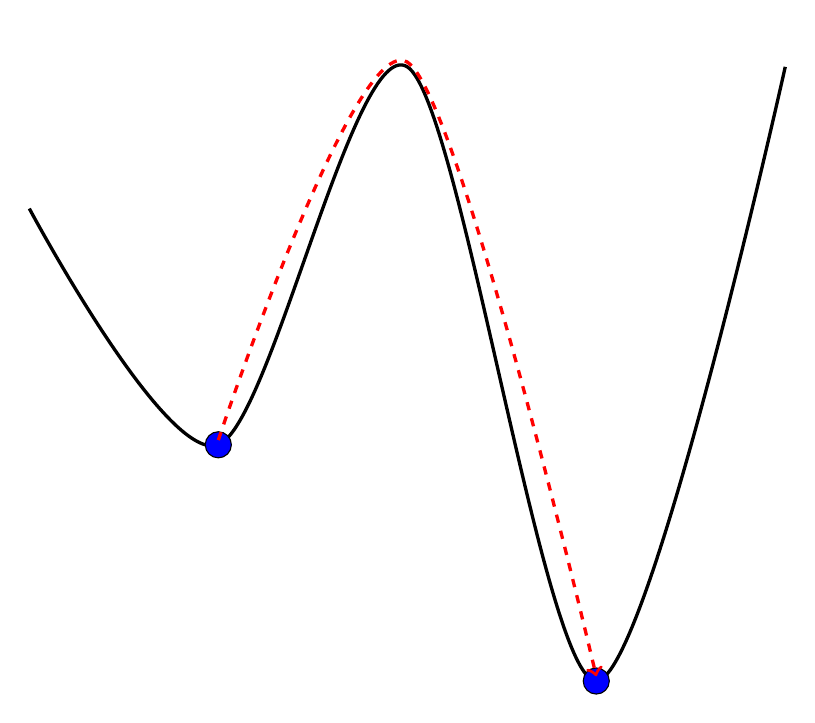
\begin{tikzpicture}[every node/.style={draw,shape=circle,fill=blue},
            scale=.6]
        \draw [very thick] plot [smooth] coordinates {(0, 0) (4, -5) (8, 3) (12, -10) (16, 3)};
        \node [fill=blue] at (4, -5) {};
        \node [fill=blue] at (12, -10) {};
        \draw [very thick, red, dashed, ->] plot [smooth] coordinates {(4, -4.9) (8, 3.1) (12, -9.9)};
        \end{tikzpicture}
    \end{frame}

    \begin{frame}
        \begin{columns}
            \begin{column}{.3\textwidth}
                \centering
                
\includegraphics[width=.95\textwidth]{./static/fire_twemoji.pdf}
            \end{column}

            \begin{column}{.3\textwidth}
                \centering
                
\includegraphics[width=.95\textwidth]{./static/sword_twemoji.pdf}
            \end{column}

            \begin{column}{.3\textwidth}
                \centering
                
\includegraphics[width=.95\textwidth]{./static/hammer_twemoji.pdf}
            \end{column}

        \end{columns}

            \hfill\tiny{(CC-BY Twitter)}
    \end{frame}

    \begin{frame}[fragile]{}
        \centering
        \texttt{conference\_scheduler/heuristics/simulated\_annealing.py}:

        \scriptsize
        \begin{minted}[linenos, 
                       firstnumber=34, 
                       frame=single]{python}
while current_energy > lower_bound and iterations <= max_iterations:

    iterations += 1
    candidate = element_from_neighbourhood(X)
    candidate_energy = objective_function(candidate)

    delta = candidate_energy - current_energy

    if (candidate_energy < best_energy and
        (acceptance_criteria is None or
         acceptance_criteria(candidate) <= acceptance_bound)):

        best_energy = candidate_energy
        best_X = candidate


    if delta < 0 or (temperature > 0 and
                 np.random.random() < np.exp(-delta / temperature)):
        X = candidate
        current_energy = candidate_energy

    temperature *= (cooldown_rate) ** iterations

        \end{minted}
\end{frame}

\begin{frame}
    \begin{center}
        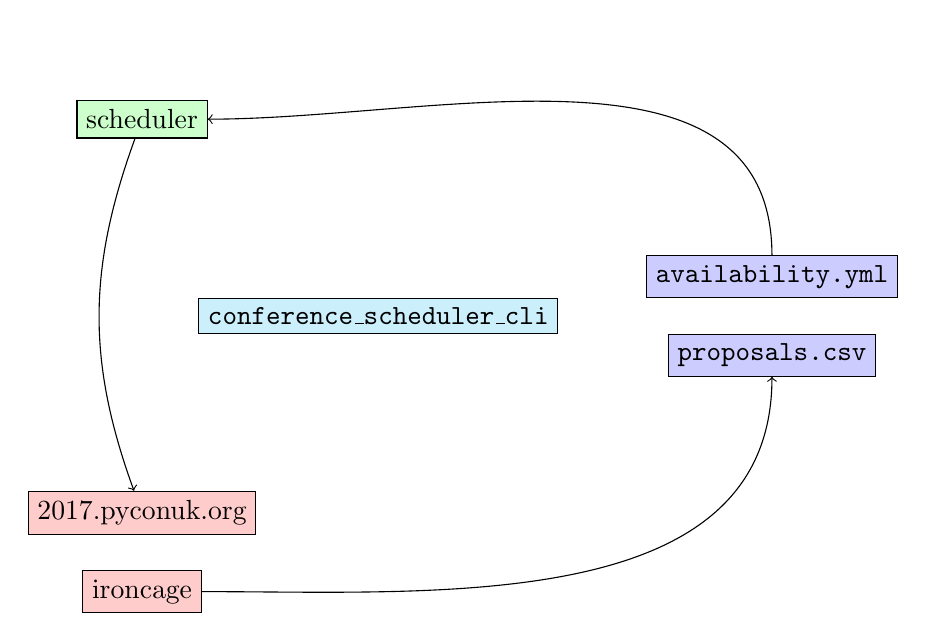
\begin{tikzpicture}
            \node [draw, fill=red!20] (ironcage) at (0, 0) {ironcage};
            \node [draw, fill=red!20] (site) at (0, 1) {2017.pyconuk.org};

            \node [draw, fill=blue!20] (availability) at (8, 4)
                {\texttt{availability.yml}};
            \node [draw, fill=blue!20] (proposals) at (8, 3)
                {\texttt{proposals.csv}};

            \node [draw, fill=green!20] (scheduler) at (0, 6) {scheduler};

            \draw (ironcage) edge[out=0, in=-90, ->] (proposals);
            \draw (availability) edge[out=90, in=0, ->] (scheduler);
            \draw (scheduler) edge[out=-110, in=110, ->] (site);

            \node [draw, fill=cyan!20] (cli) at (3, 3.5)
                {\texttt{conference\_scheduler\_cli}};
        \end{tikzpicture}

        \url{github.com/PyconUK}
    \end{center}
\end{frame}

\begin{frame}
    \Large
    \begin{center}
        \url{conference-scheduler.readthedocs.io}

        \url{github.com/PyconUK}

        \href{https://twitter.com/drvinceknight}{@drvinceknight}
    \end{center}
\end{frame}

\end{document}
